\clearpage
\section{Calibration}\label{sec:cal}
After adjusting the PMT voltage and threshold voltage, the setup should function as expected. An overnight data taking is performed and all data has been stored. The tutor mentioned that the calibration option 1 is not working properly, so the second option is chosen. 

\begin{figure}[ht]
	\centering
	\begin{subfigure}[t]{0.6\textwidth}
	\begin{center}
	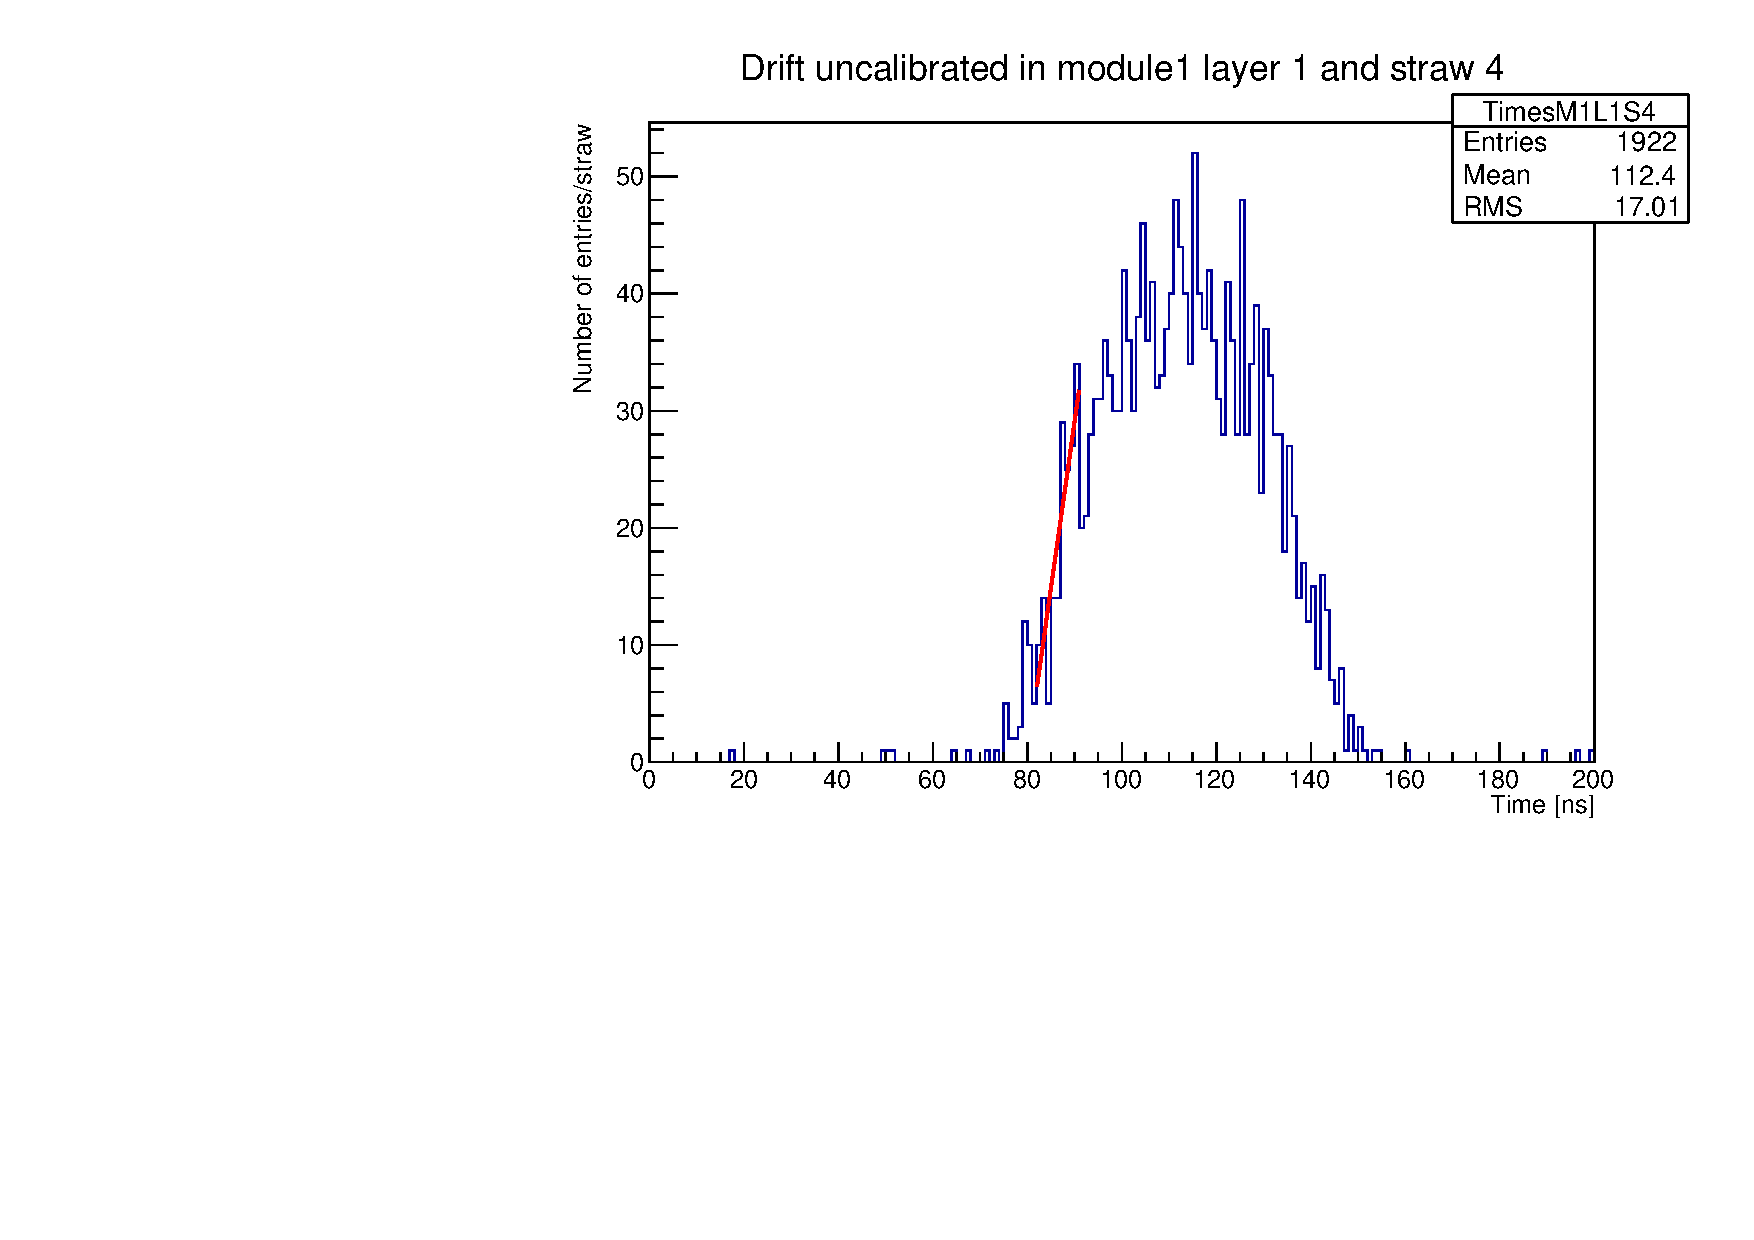
\includegraphics[width=\linewidth]{t0_fit_b.pdf}
	\end{center}
	\caption{Before calibration. Red line is a fit.}
	\end{subfigure}
	\begin{subfigure}[t]{0.6\textwidth}
	\begin{center}
	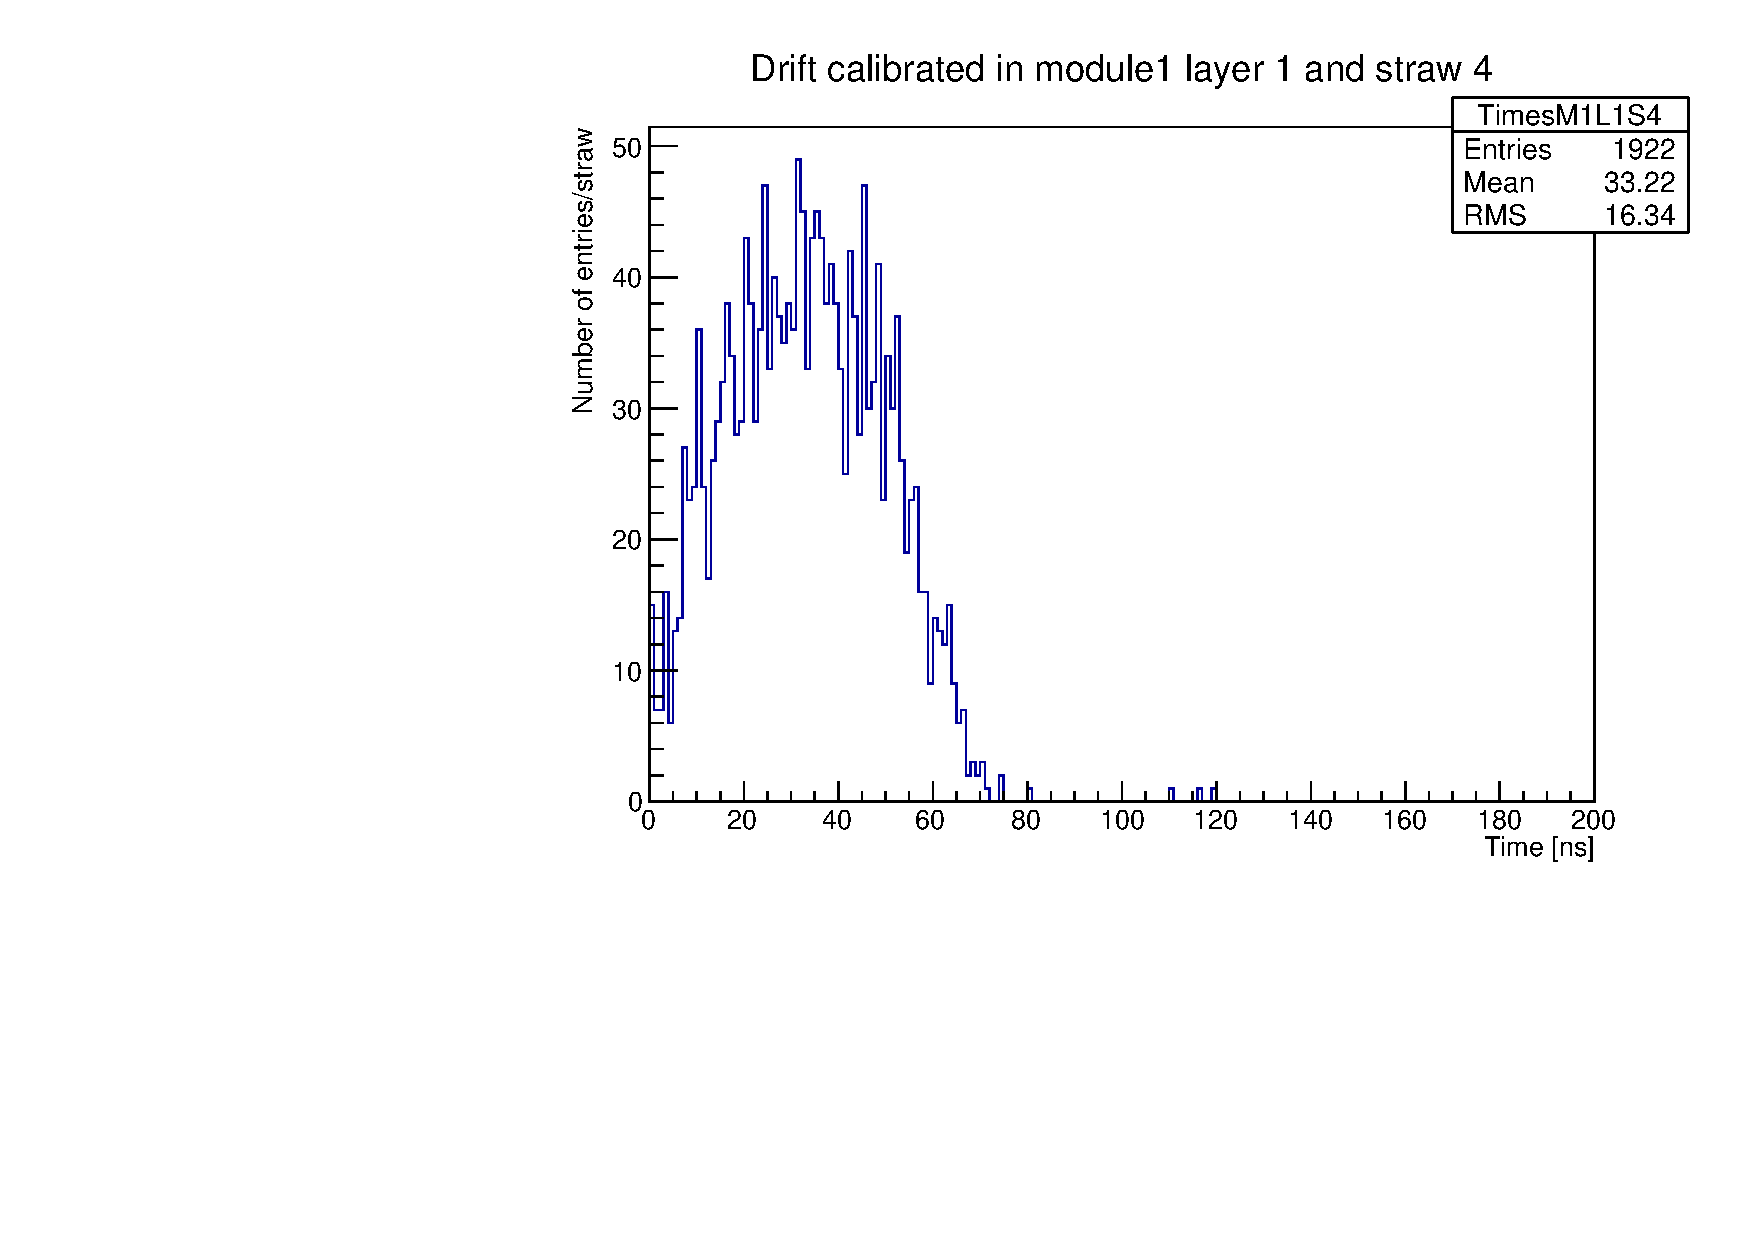
\includegraphics[width=\linewidth]{t0_fit_a.pdf}
	\end{center}
	\caption{After calibration}
	\end{subfigure}
	\caption{Drift time spectrum before and after calibration.}%
	\label{fig:drift-time}
\end{figure}
The calibration is done straw-by-straw using the data. One part of the data is used to map out the drift time spectrum for each straw. During the calibration, the program will try to shift the drift time, so that it starts at zero time. Exemplar spectra can be found in figure~\ref{fig:drift-time}. During the calibration a fit is done to the "leading" edge of the drift spectrum. The initial time $t_0$ is then set the intersection point of the fit line with horizontal axis.

The calibration is performed with \num{300 000} events using the program \verb|StyxCalibration| (with \verb|--no-clean| and \verb|--all| options). The calibration method is specified with \verb|-A CalibStrawByStraw|. After execution of the command, corresponding \verb|root| and \verb|txt| file are generated.

In the generated \verb|root| file, there are two plots of particular interest: \verb|Uncalibrated/Layers2D| and \verb|Calibrated/Layers2D|. These plots show the drift spectra for each straw in one particular module and layer before and after calibration. Some examples are figure~\ref{fig:layer2D-1},~\ref{fig:layer2D-2}, and~\ref{fig:layer2D-3}.
\begin{figure}[ht]
	\centering
	\begin{subfigure}[t]{0.7\textwidth}
	\begin{center}
	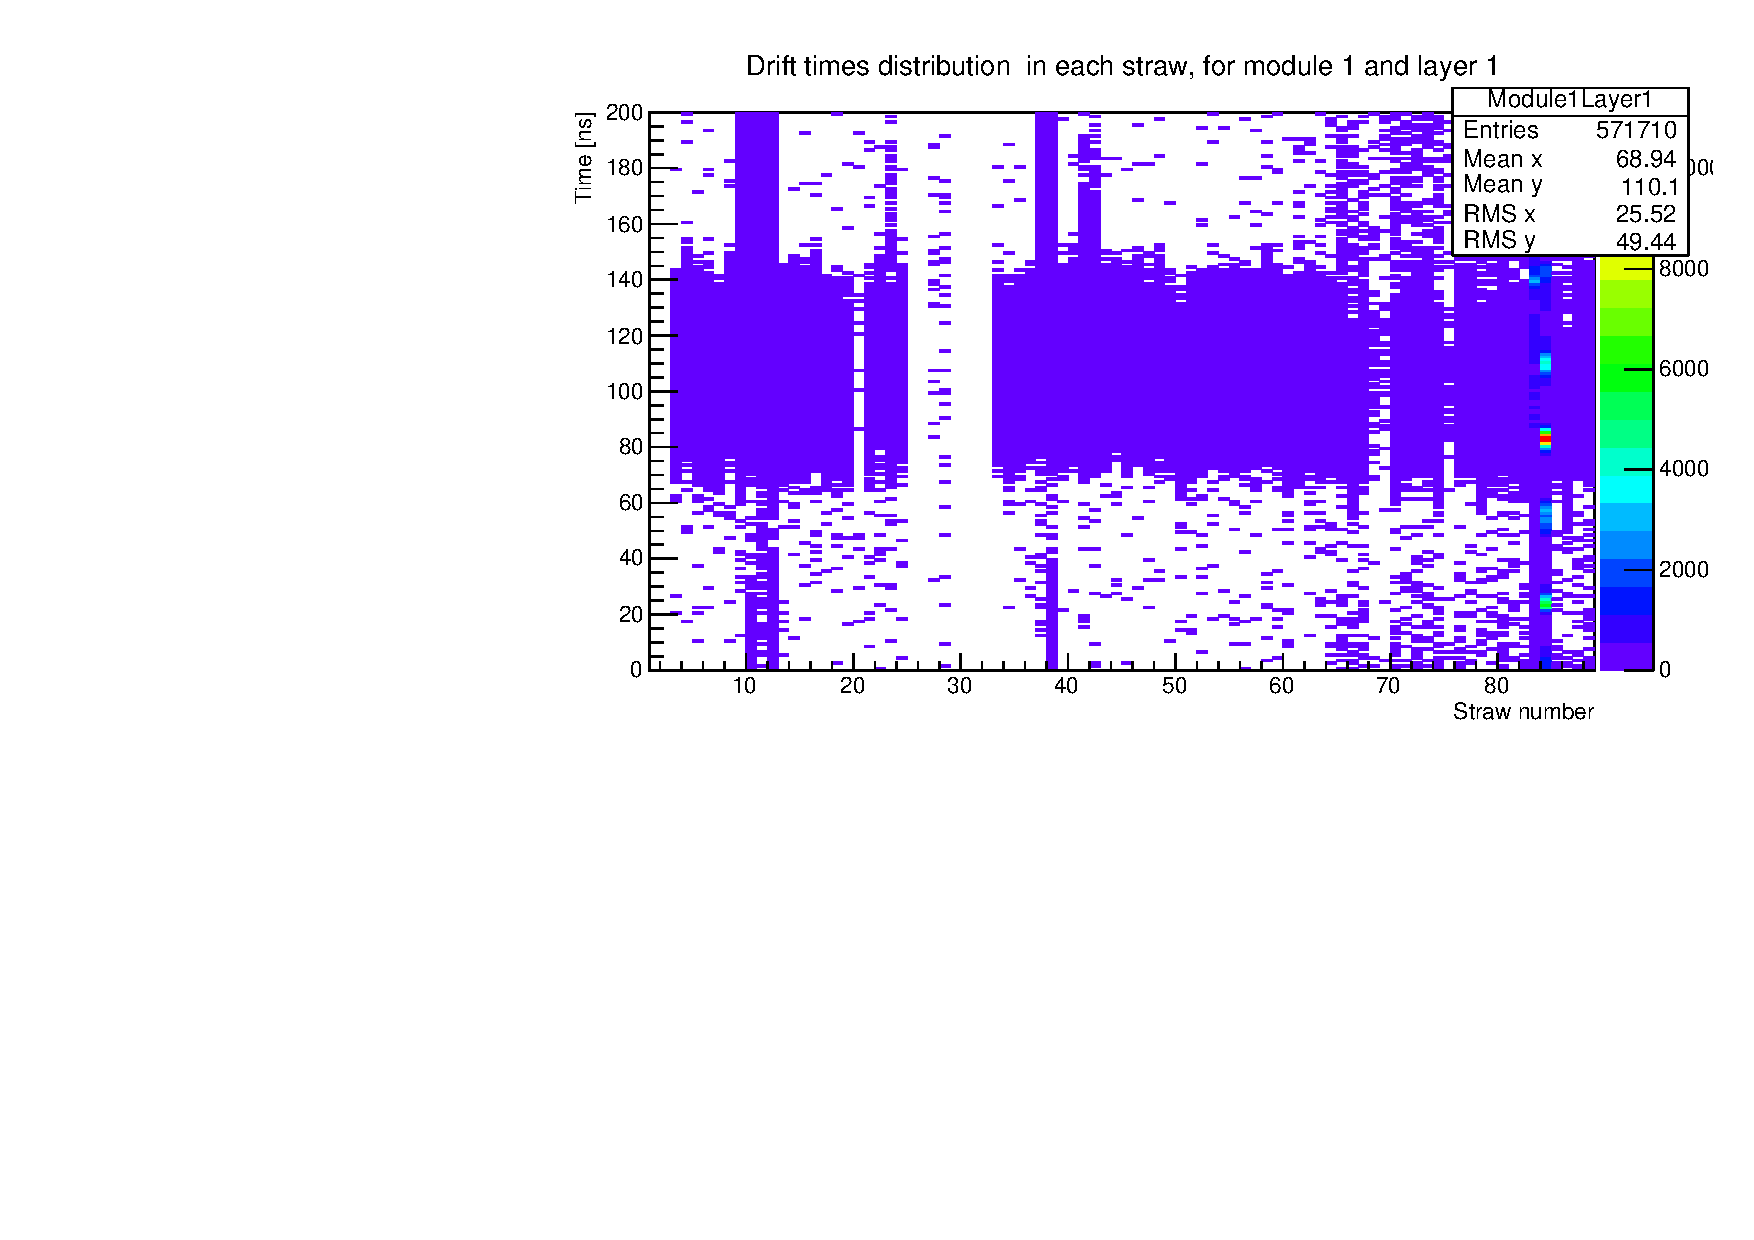
\includegraphics[width=\linewidth]{cal-b1.pdf}
	\end{center}
	\caption{Before calibration. }
	\end{subfigure}
	\begin{subfigure}[t]{0.7\textwidth}
	\begin{center}
	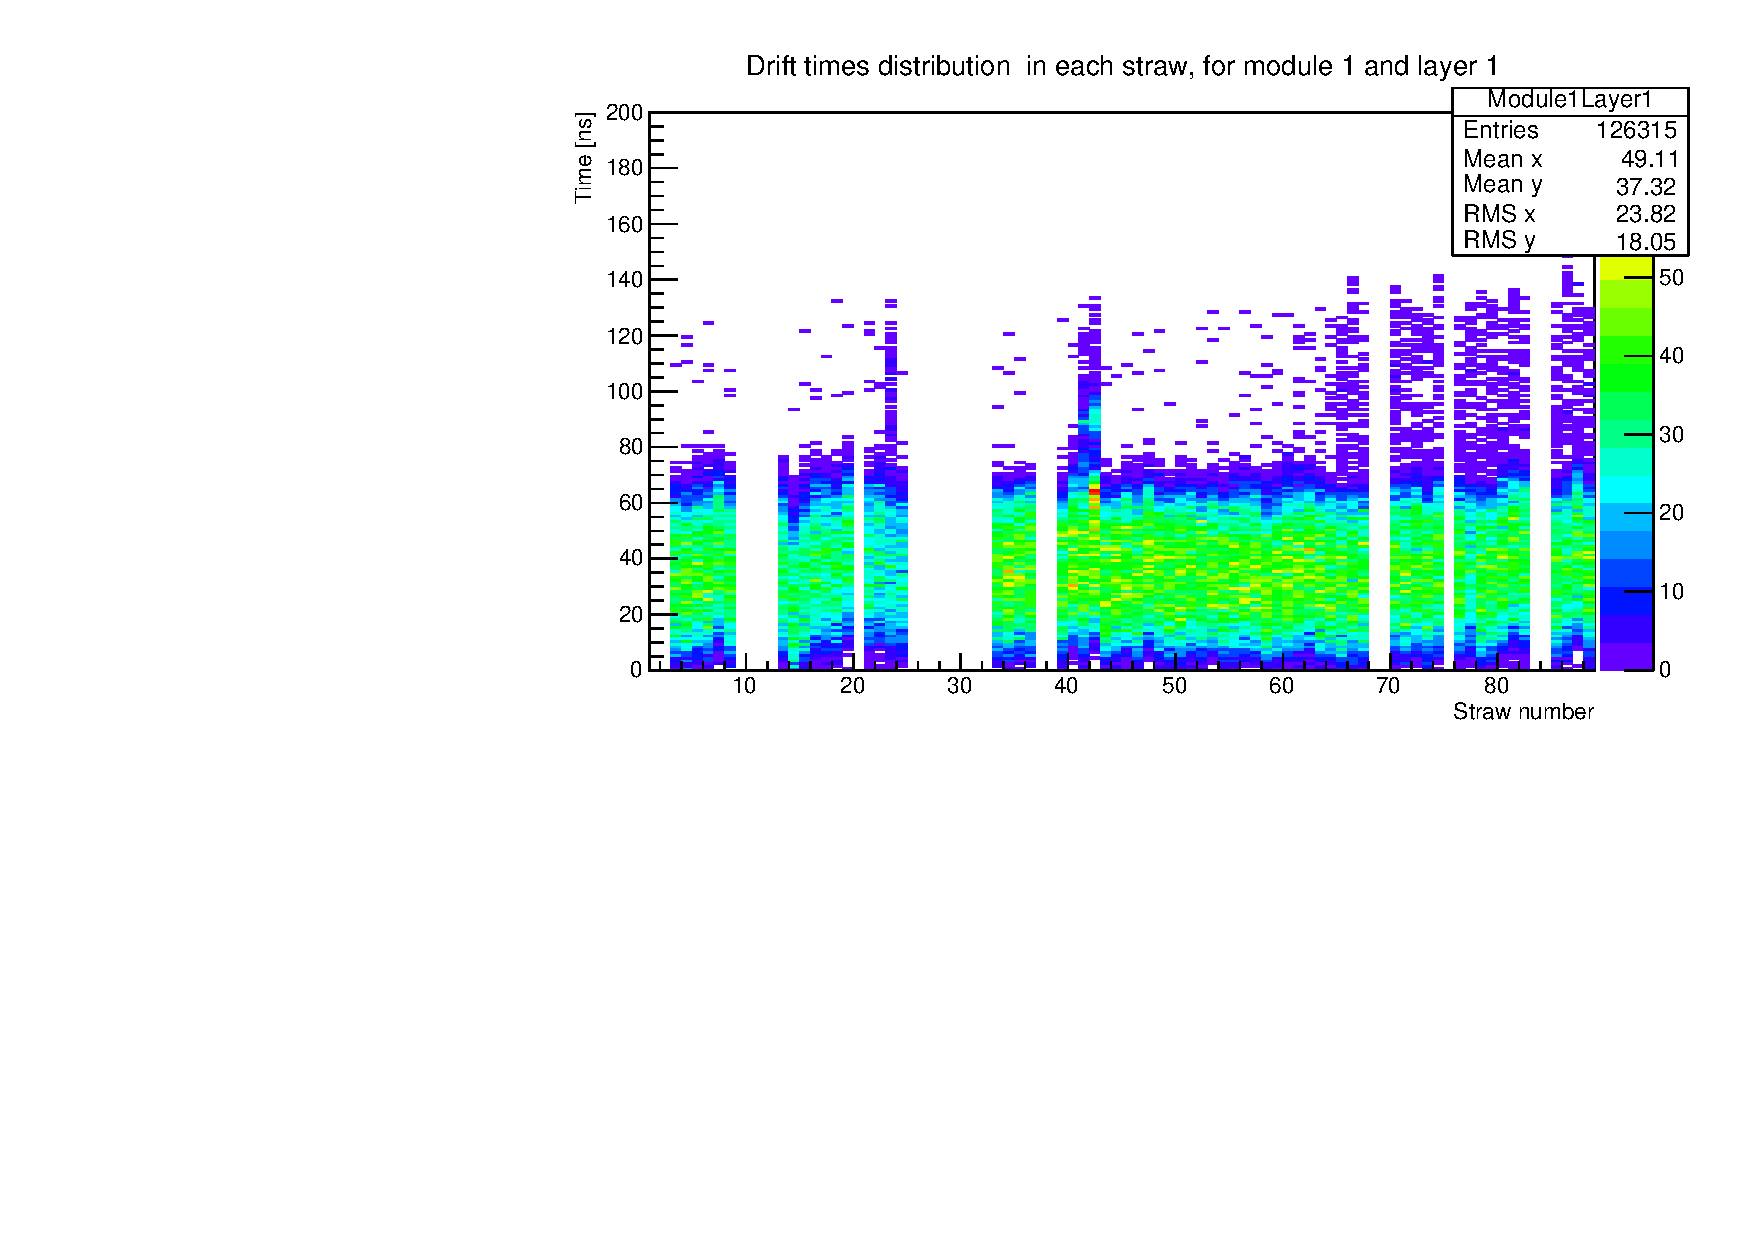
\includegraphics[width=\linewidth]{cal-a1.pdf}
	\end{center}
	\caption{After calibration}
	\end{subfigure}
	\caption{Drift time spectra for all straws in module $1$ and layer $1$ before and after calibration.}%
	\label{fig:layer2D-1}
\end{figure}
\begin{figure}[ht]
	\centering
	\begin{subfigure}[t]{0.7\textwidth}
	\begin{center}
	\includegraphics[width=\linewidth]{cal-b2.pdf}
	\end{center}
	\caption{Before calibration. }
	\end{subfigure}
	\begin{subfigure}[t]{0.7\textwidth}
	\begin{center}
	\includegraphics[width=\linewidth]{cal-a2.pdf}
	\end{center}
	\caption{After calibration}
	\end{subfigure}
	\caption{Drift time spectra for all straws in module $2$ and layer $1$ before and after calibration.}%
	\label{fig:layer2D-2}
\end{figure}
\begin{figure}[ht]
	\centering
	\begin{subfigure}[t]{0.7\textwidth}
	\begin{center}
	\includegraphics[width=\linewidth]{cal-b3.pdf}
	\end{center}
	\caption{Before calibration. }
	\end{subfigure}
	\begin{subfigure}[t]{0.7\textwidth}
	\begin{center}
	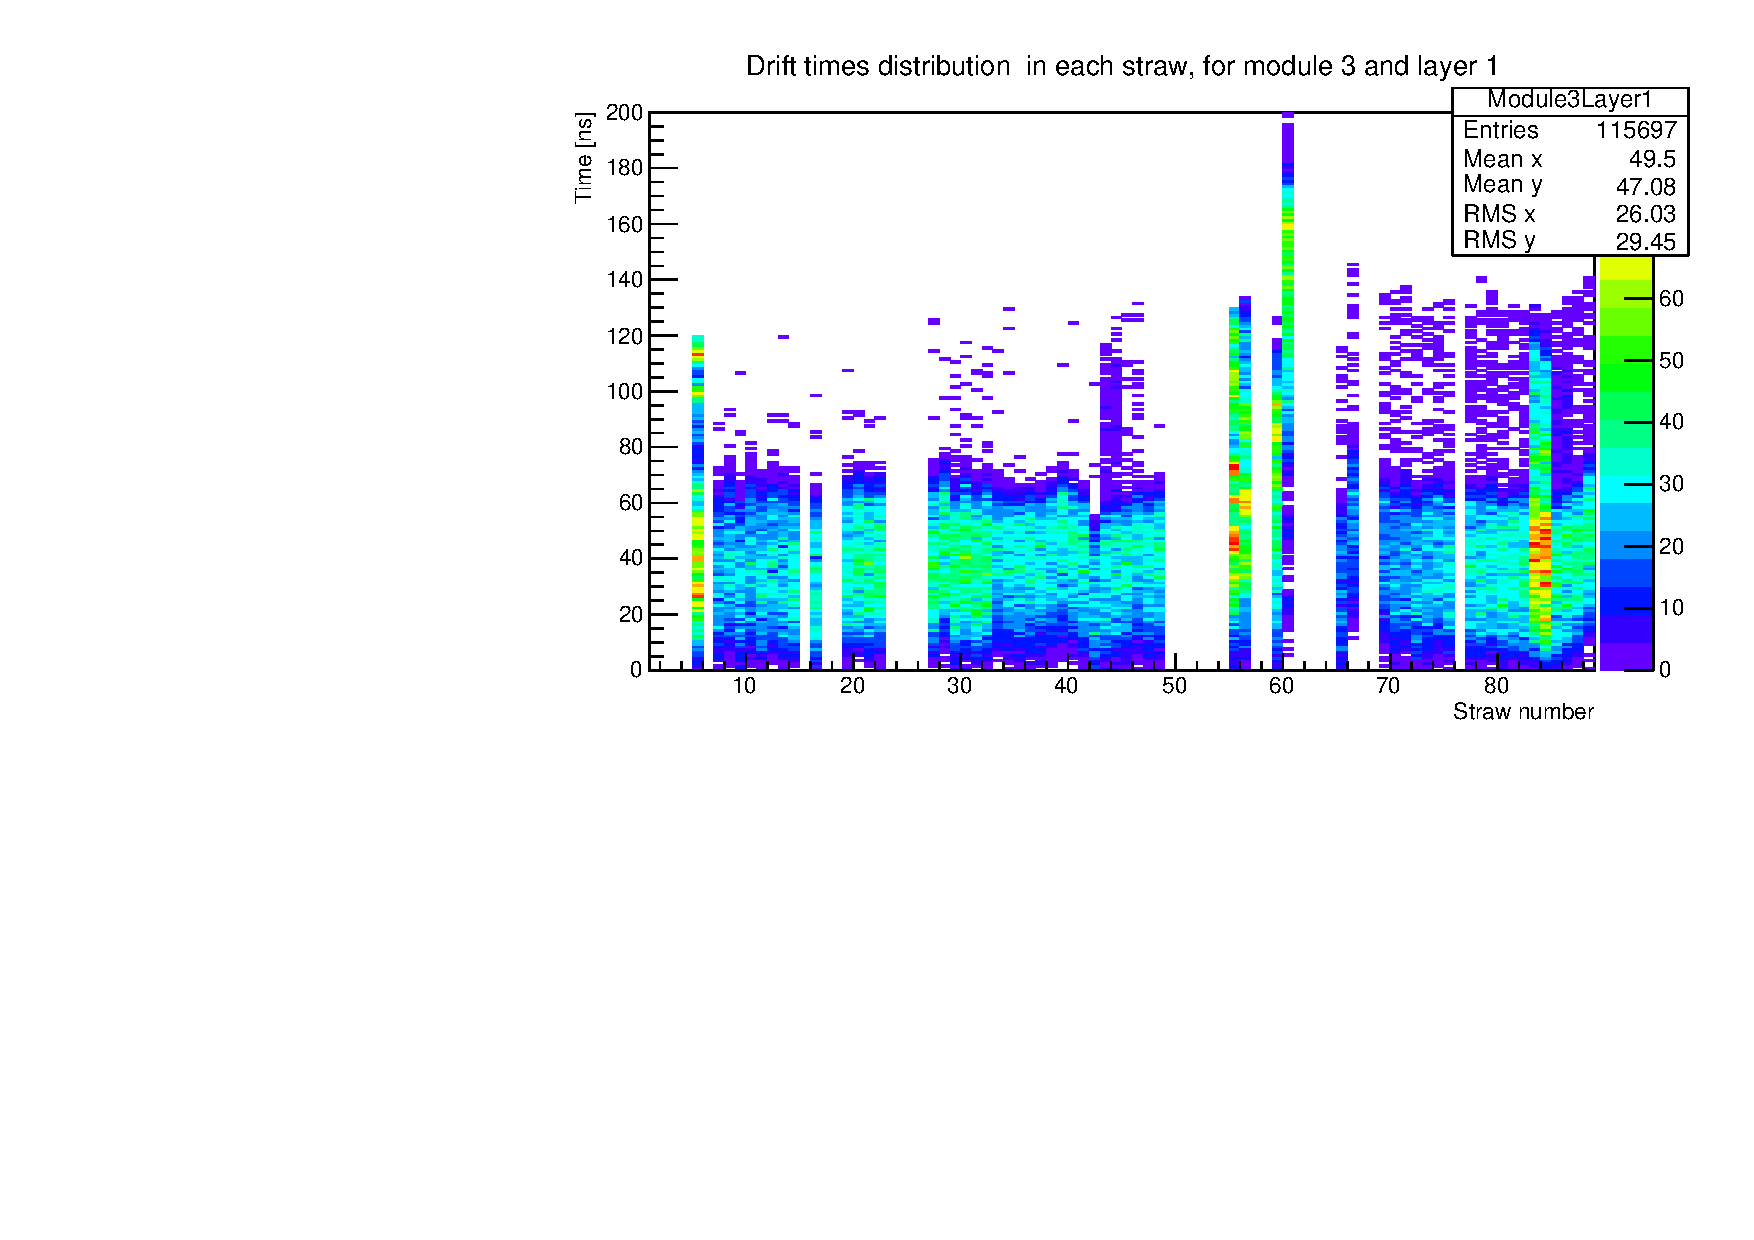
\includegraphics[width=\linewidth]{cal-a3.pdf}
	\end{center}
	\caption{After calibration}
	\end{subfigure}
	\caption{Drift time spectra for all straws in module $3$ and layer $1$ before and after calibration.}%
	\label{fig:layer2D-3}
\end{figure}

\clearpage
By comparison of these plots, we see that the calibration works normally for most straws. Before the calibration, there are no particular "hot" time (interval of time with clear peak in event counts) and events are rather scattered in time. But after, events are properly aligned with each other and there is a clear peak at $t\approx\SI{40}{\nano\second}$. One can also notice that some straws don't have a lot of outputs or even no output at all. These straws should be marked as "dead". Sometimes, even after calibration, the drift spectra cannot get into the shape we expect, such as straw $15$ and $16$ in figure~\ref{fig:layer2D-2}. This can be understood as the straws cannot be properly calibrated. The exact reason of failing calibration is still yet unknown. These certainly should not be used for the track analysis and these straws are marked as "hot" or "continuous". 

The aforementioned labels to each straws can be mapped onto the cross section of the detectors, see figure~\ref{fig:strawMasks}.
\begin{figure}[ht]
	\centering
	\includegraphics[width=0.95\linewidth]{strawMasks.pdf}
	\caption{Straw masks. Note that the numbering should start from bottom. It means that the bottom module is module $1$, the same for layer numbering. Dead straws are in orange.}%
	\label{fig:strawMasks}
\end{figure}

With the masks, one can even simulate the events. By looking at it, we are able to gain further insight to the reconstruction process (algorithms). For example, with number of events at $20$ and number of tracks at $3$, one has figure~\ref{fig:simu}. In the figure, red circles should be the expected position of the track only using one straw on one layer. When signals get correlated in the same module, possible tracks (green line) can be drawn. Then the signals from all three modules get combined together and a clear track (blue dotted lines) can be reconstructed.
\begin{figure}[ht]
	\centering
	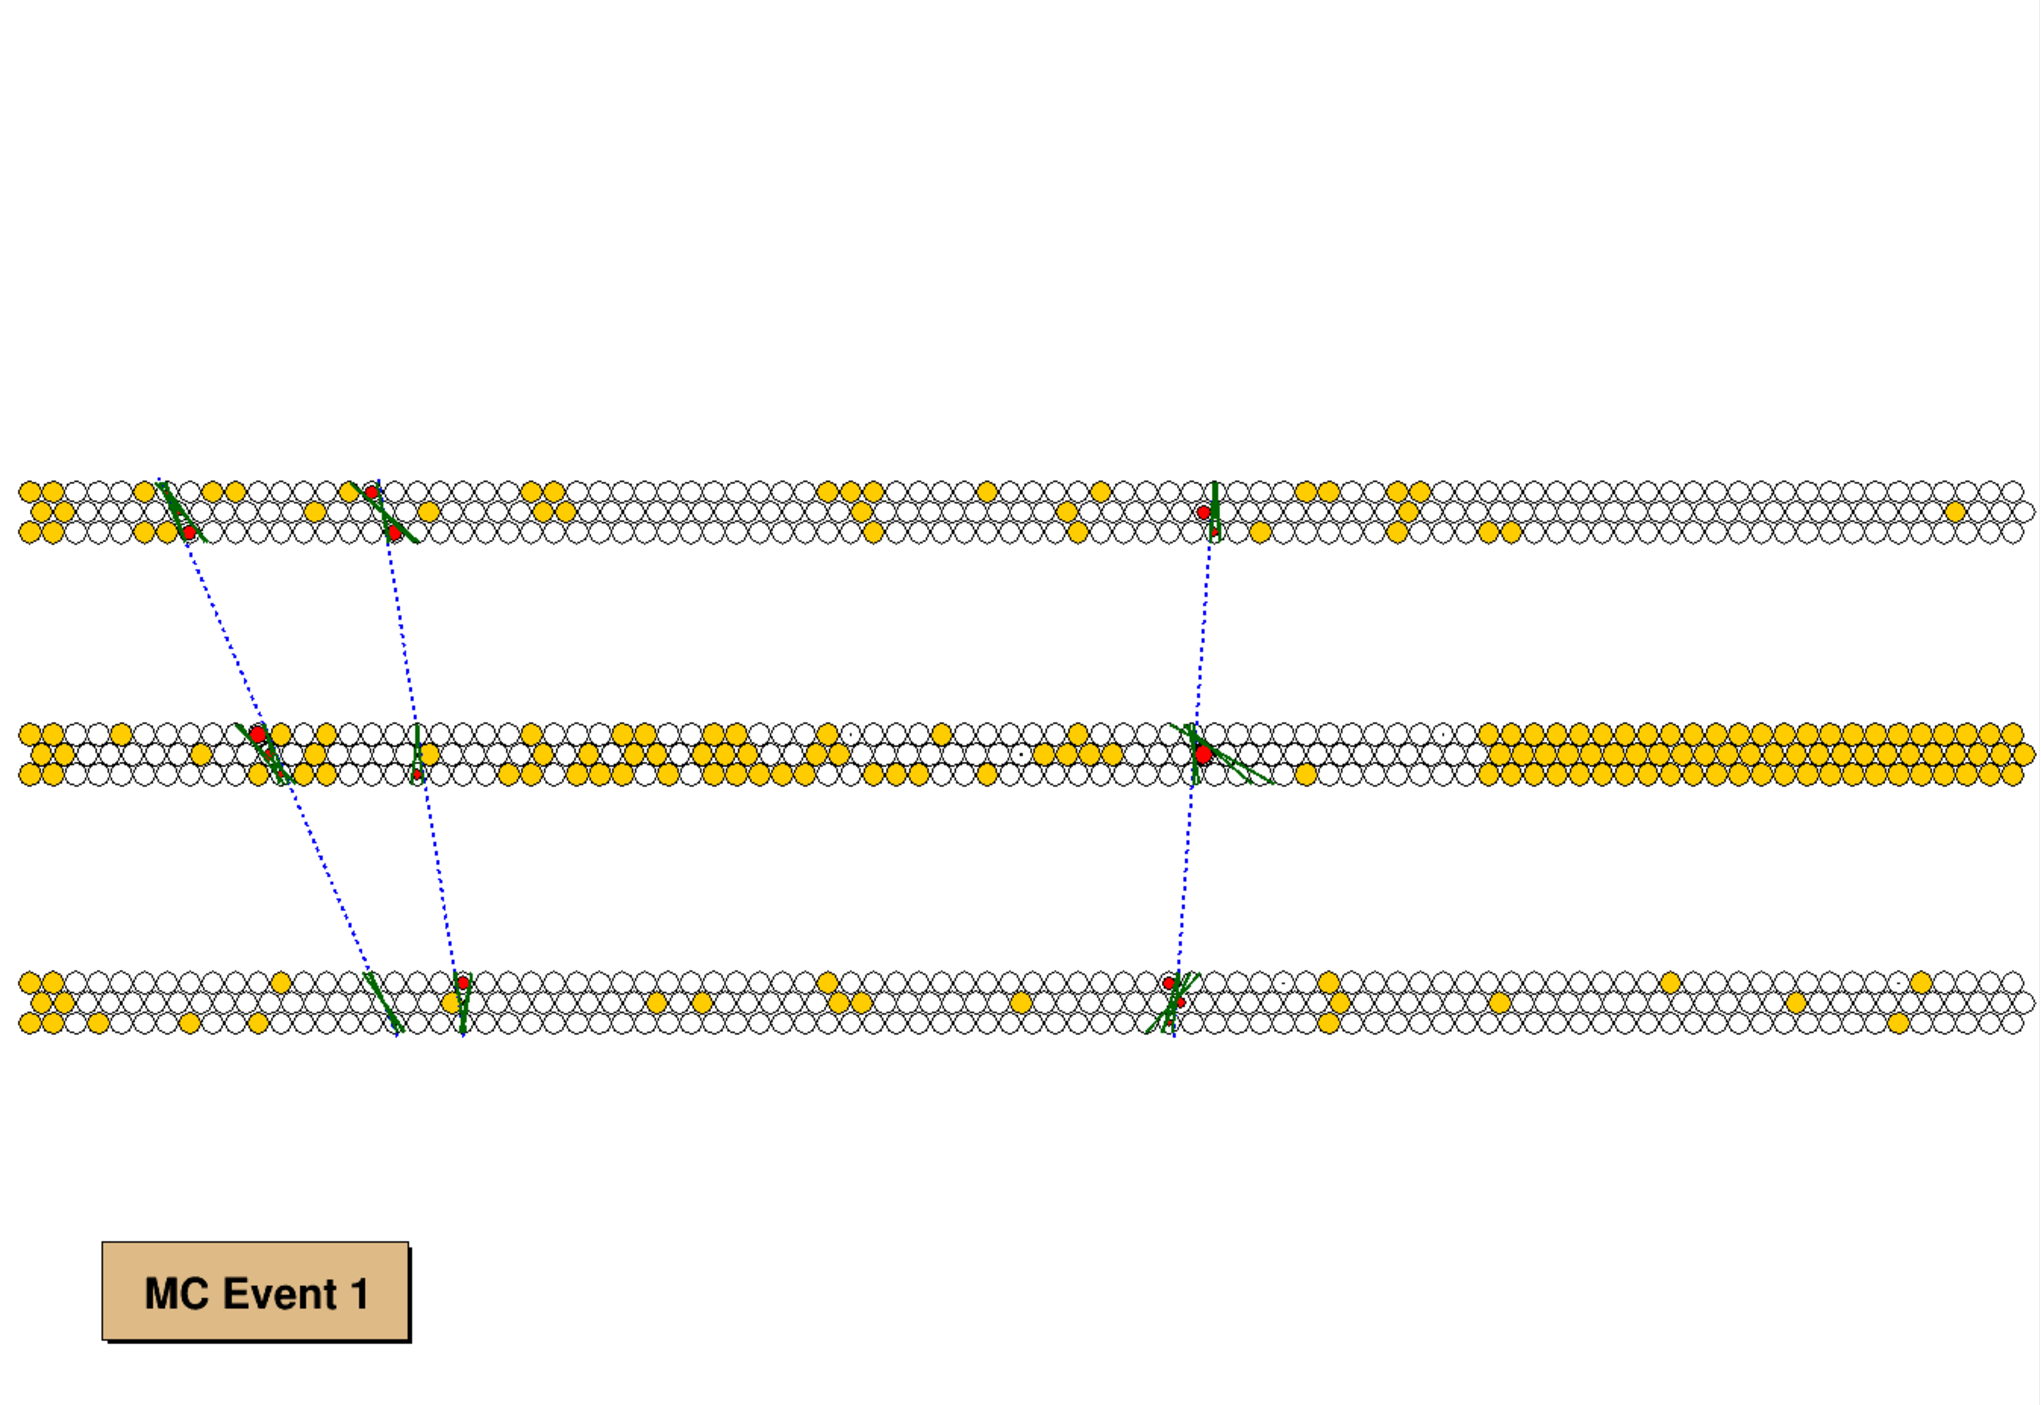
\includegraphics[width=0.9\linewidth]{Simulation3.pdf}
	\cprotect\caption{Simulation of events with \verb|Nevents=20| and \verb|Ntracks=3|. Orange straws are the straws marked as "dead".}%
	\label{fig:simu}
\end{figure}
